\section{Event selection}\label{sec:eventselection}

For all event selections presented later on
the main backgrounds are
\begin{description}
\item[Top pairs] Top pair events are the dominant SM background to the search, 
    since they contain real opposite sign leptons, missing transverse energy and
    a non negligible jet activity. This background is estimated by the opposite
    flavour subtraction.
\item[Z+jets] Events with a $Z$ Boson contain two opposite sign leptons and 
    can contain a high jet activity, but the missing transverse energy is always
   instrumental and therefore the background can be reduced completely.
   This backround can be estimated using the JZB method~\cite{kostas}
   and is found to be very small in the signal region.
\item[W+jets] Events with a $W$ Boson contain real missing transverse energy and
    can contain a high jet activity, but do only contain one lepton.
    Therefore the background can be measured using the fake lepton component.
    This background is estimated by the isolation template method.
\item[Diboson] Events with two gauge bosons do contribute to the background.
    Due to the low cross-section of the process their contribution is found
    to be negligible. This background is estimated from MC.
\item[QCD] Although the di-jet cross-section is huge, this background is found to 
    be negligible in MC, since all cuts act very well on QCD (no isolated leptons,
    no missing transverse energy and  a steeply falling \HT distribution). 
    This background is estimated by the isolation template method.
\end{description}

\subsection{Preselection}

For now we select only events using the lepton trigger selection,
but lower \pT leptons can be added without any changes to the 
presented methods.
We start from a common preselection defined as
\begin{itemize}
\item Two leptons of opposite sign with the thresholds
of $p_T>20$~GeV for the hardest and $p_T>10$~GeV for 
the second lepton.
\item At least two jets and a $\HT>100$~GeV.
\item A missing transverse energy of at least $\MET>100$~GeV.
\end{itemize}

The region is expected to be dominated by events with di-leptonic
top decays. The yields in data and simulation are given in
Tab.~\ref{tab:presel}

\begin{table}[htb]
\begin{center}
\caption{\label{tab:presel}\protect Summary of number of events expected from Monte Carlo simulations in 
the signal region of $H_T> 100$~GeV and $\MET> 100$~GeV. The errors reflect the Monte Carlo statistics only.}
\begin{tabular}{l|ccc|c}
\hline
Process           & $ee$       & $\mu\mu$     & $e\mu$   & total   \\
\hline\hline
$W+\textrm{jets}$ &$0.0 \pm 0.0$&$0.0 \pm 0.0$&$0.0 \pm 0.0$&$0.0 \pm 0.0$\\
$Z\rightarrow ll+\textrm{jets}$&$0.16 \pm 1.76$&$0.76 \pm 2.05$&$0.04 \pm 1.86$&$0.95 \pm 3.28$\\
$Z \rightarrow \tau\tau$&$0.27 \pm 0.89$&$0.87 \pm 1.08$&$1.18 \pm 1.17$&$2.33 \pm 1.82$\\
$t\bar{t}$&$33.49 \pm 1.3$&$43.98 \pm 1.49$&$77.11 \pm 1.97$&$154.58 \pm 2.8$\\
\hline
Total background&$33.92 \pm 2.36$&$45.61 \pm 2.76$&$78.33 \pm 2.95$&$157.86 \pm 4.68$\\\hline
\hline
Data  & 44 & 47 & 101 & 192 \\
\hline\hline
%LM0               &$3.41 \pm 0.17$&$3.91 \pm 0.17$&$4.52 \pm 0.14$&$11.84 \pm 0.42$ \\
%LM1               &$1.64 \pm 0.04$&$2.02 \pm 0.04$&$1.01 \pm 0.03$&$4.64 \pm 0.07$ \\
%\hline
\end{tabular}
\end{center}
\end{table}


\subsection{Definition of the signal regions}

To be prepared for a much larger luminosity we
define tighter signal regions for an
intgrated luminosity of up to 1~fb$^{-1}$.

\subsubsection{2010 signal region}
For reference we keep the signal region used in 2010. It is defined by
tightening both $\HT$ and \MET from the preselection region
to $\HT>350$~GeV and $\MET>150$~GeV.

\begin{figure}[hbtp]
  \subfigure[]{\label{fig:MET2010}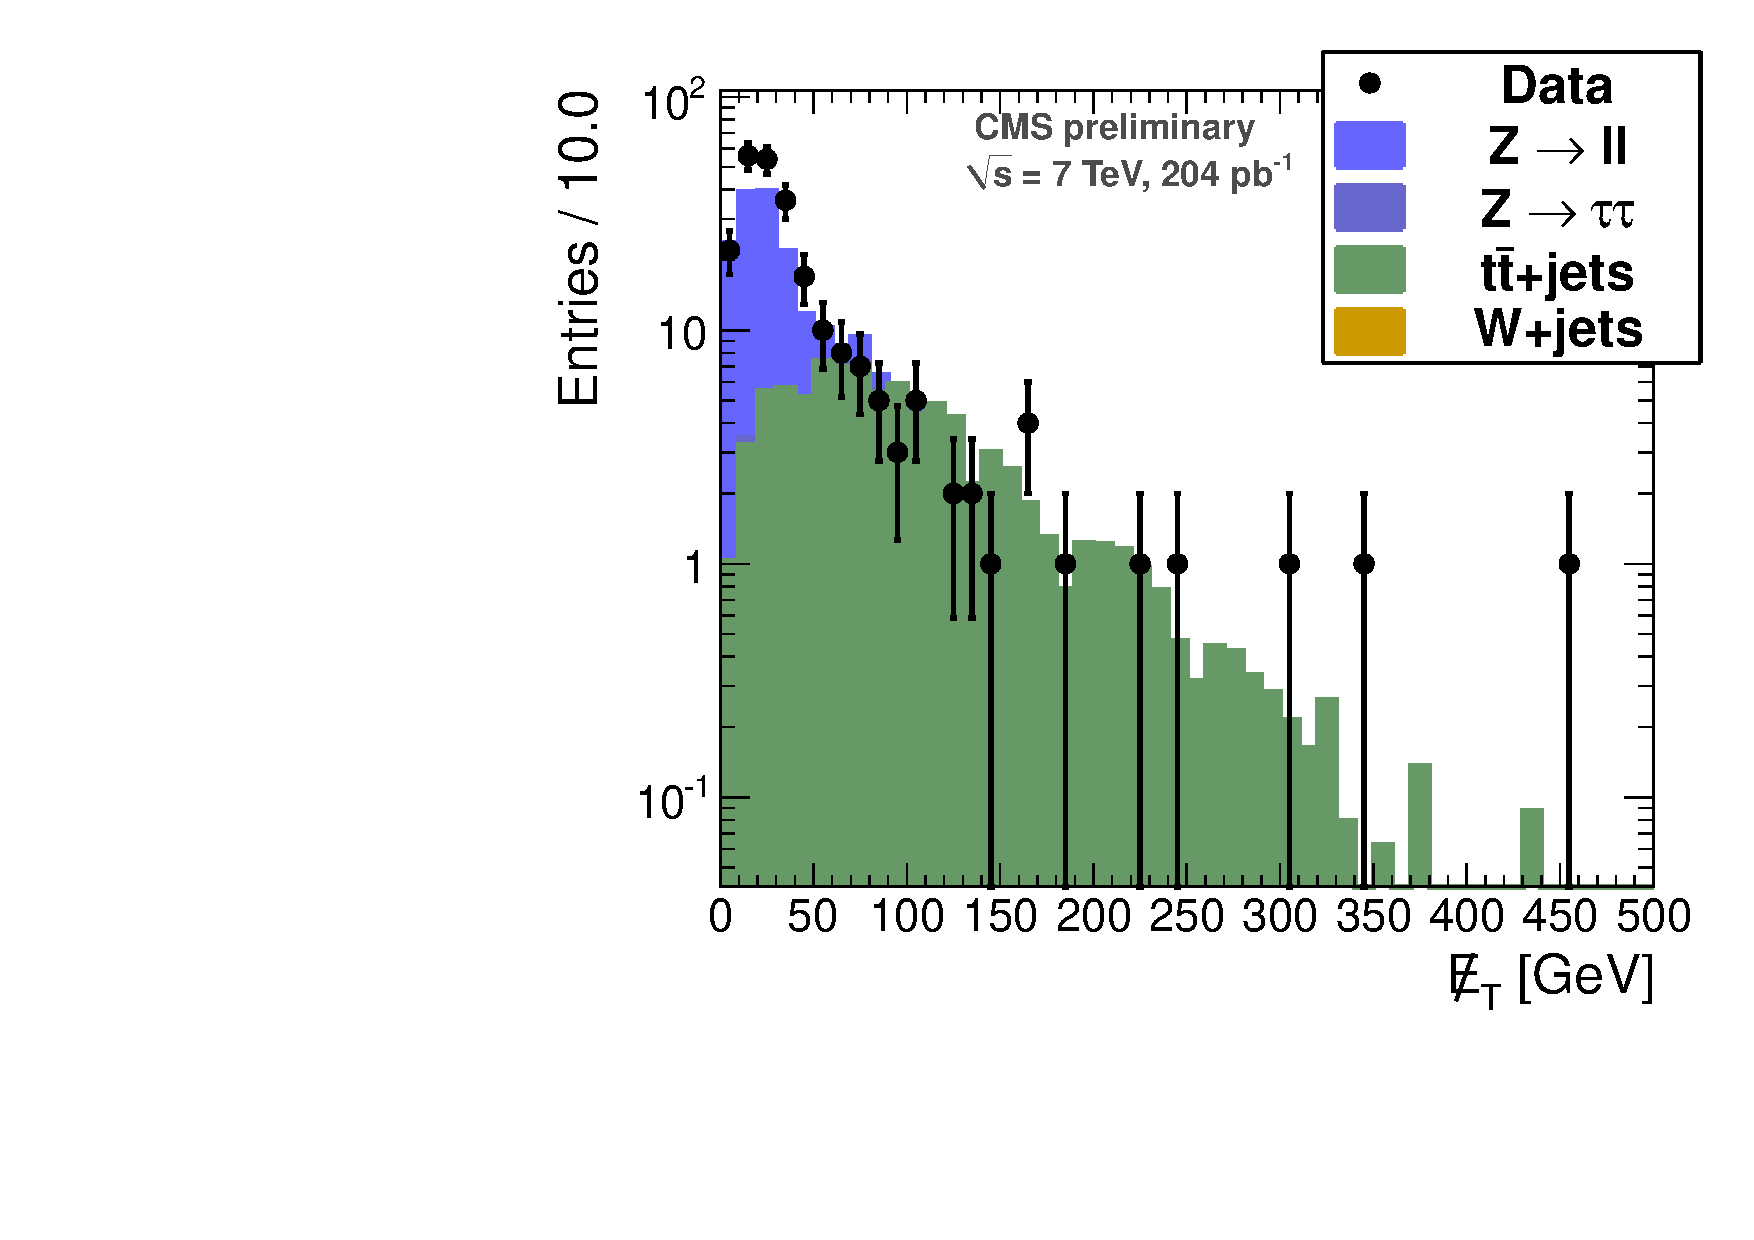
\includegraphics[width=0.79\textwidth]{Summer11_07_MC_pfLeptSusyCuts_Data_MET_2010.pdf}}\hfill
  \caption{\MET distribution for all events passing di-lepton selection and satisy $\HT> 350$~GeV. For the final \MET selection (150)~GeV the selection is dominated by $t\bar{t}$.}
\end{figure}

The \MET distribution after application of the \HT
cut is shown in Fig~\ref{fig:MET2010} and
the yield split by flavour for a cut at 150~GeV is listed in Tab.~\ref{tab:2010}.
It is seen that the yield in simulation is higher
than in the data for this selection.

\begin{table}[htb]
\begin{center}
\caption{\label{tab:2010}\protect Summary of number of events expected from Monte Carlo simulations in 
the signal region of $H_T> 350$~GeV and $\MET> 150$~GeV. The errors reflect the Monte Carlo (scaled
    to 204~\pbi) statistics only.}
\begin{tabular}{l|ccc|c}
\hline
Process           & $ee$       & $\mu\mu$     & $e\mu$   & total   \\
\hline\hline
$W+\textrm{jets}$&$0.0 \pm 0.0$&$0.0 \pm 0.0$&$0.0 \pm 0.0$&$0.0 \pm 0.0$\\
$Z\rightarrow ll+\textrm{jets}$&$0.0 \pm 1.97$&$0.0 \pm 1.97$&$0.0 \pm 1.97$&$0.0 \pm 0.27$\\
$Z \rightarrow \tau\tau$&$0.0 \pm 1.0$&$0.0 \pm 1.0$&$0.0 \pm 1.0$&$0.0 \pm 0.27$\\
$t\bar{t}$&$3.44 \pm 0.42$&$4.26 \pm 0.47$&$7.46 \pm 0.63$&$15.17 \pm 0.9$\\
\hline
Total background&$3.44 \pm 2.25$&$4.26 \pm 2.26$&$7.46 \pm 2.3$&$15.17 \pm 0.98$\\
\hline
Data  & 3 & 3 & 4 & 10 \\
\hline\hline
%LM0               &$3.41 \pm 0.17$&$3.91 \pm 0.17$&$4.52 \pm 0.14$&$11.84 \pm 0.42$ \\
%LM1               &$1.64 \pm 0.04$&$2.02 \pm 0.04$&$1.01 \pm 0.03$&$4.64 \pm 0.07$ \\
%\hline
\end{tabular}
\end{center}
\end{table}

\subsubsection{High \HT signal region}

A signal region with high \HT is defined by tightening the $\HT$ 
from the preselection region to $\HT>600$~GeV and $\MET>100$~GeV.

\begin{figure}[hbtp]
  \subfigure[]{\label{fig:METHighHT}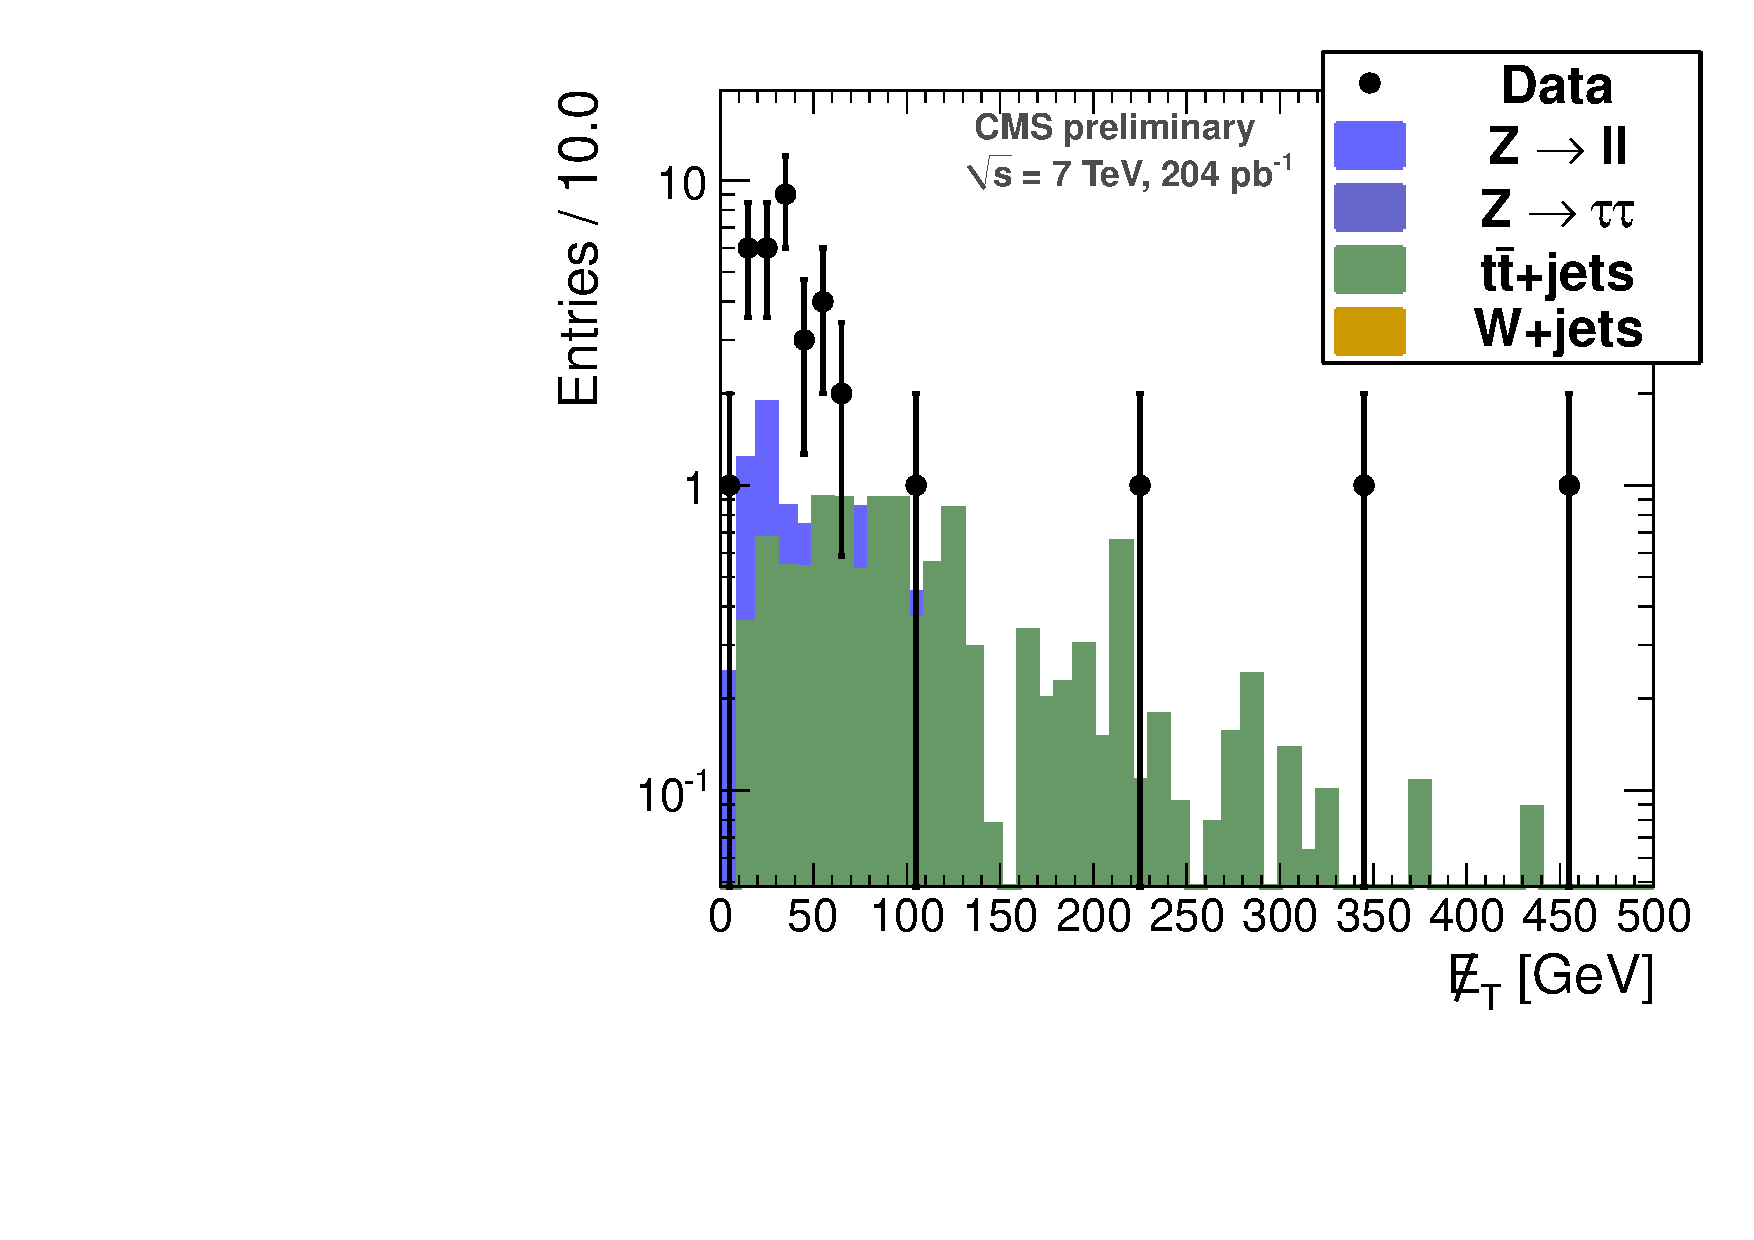
\includegraphics[width=0.79\textwidth]{Summer11_07_MC_pfLeptSusyCuts_Data_MET_HighHT.pdf}}\hfill
  \caption{\MET distribution for all events passing di-lepton selection and satisfy $\HT> 600$~GeV. For the final \MET selection (100)~GeV the selection is dominated by $t\bar{t}$.}
\end{figure}

The \MET distribution after application of the \HT
cut is shown in Fig~\ref{fig:METHighHT} and
the yield split by flavour for a cut at 100~GeV is listed in Tab.~\ref{tab:HighHT}.
It is seen that the yield in the data is lower than expected
from the simulation.

\begin{table}[htb]
\begin{center}
\caption{\label{tab:HighHT}\protect Summary of number of events expected from Monte Carlo simulations in 
the signal region of $H_T> 600$~GeV and $\MET> 100$~GeV. The errors reflect the Monte Carlo (scaled
    to 204~\pbi) statistics only.}
\begin{tabular}{l|ccc|c}
\hline
Process           & $ee$       & $\mu\mu$     & $e\mu$   & total   \\
\hline\hline
$W+\textrm{jets}$&$0.0 \pm 0.0$&$0.0 \pm 0.0$&$0.0 \pm 0.0$&$0.0 \pm 0.0$\\
$Z\rightarrow ll+\textrm{jets}$&$0.08 \pm 1.47$&$0.0 \pm 1.97$&$0.0 \pm 1.97$&$0.08 \pm 3.15$\\
$Z \rightarrow \tau\tau$&$0.0 \pm 1.0$&$0.0 \pm 1.0$&$0.0 \pm 1.0$&$0.0 \pm 0.27$\\
$t\bar{t}$&$1.11 \pm 0.23$&$1.69 \pm 0.31$&$2.7 \pm 0.41$&$5.5 \pm 0.56$\\
\hline
Total background &$1.19 \pm 1.8$&$1.69 \pm 2.23$&$2.7 \pm 2.25$&$5.58 \pm 3.22$\\
\hline
Data  & 2 & 0 & 2 & 4 \\
\hline\hline
%LM0               &$3.41 \pm 0.17$&$3.91 \pm 0.17$&$4.52 \pm 0.14$&$11.84 \pm 0.42$ \\
%LM1               &$1.64 \pm 0.04$&$2.02 \pm 0.04$&$1.01 \pm 0.03$&$4.64 \pm 0.07$ \\
%\hline
\end{tabular}
\end{center}
\end{table}


\subsubsection{High \MET signal region}

A signal region with high \MET is defined by slightly tightening the $\HT$ 
and a much tighter $\MET$ selection compared to the pre-selection region
to $\HT>250$~GeV and $\MET>250$~GeV.

\begin{figure}[hbtp]
  \subfigure[]{\label{fig:METHighHT}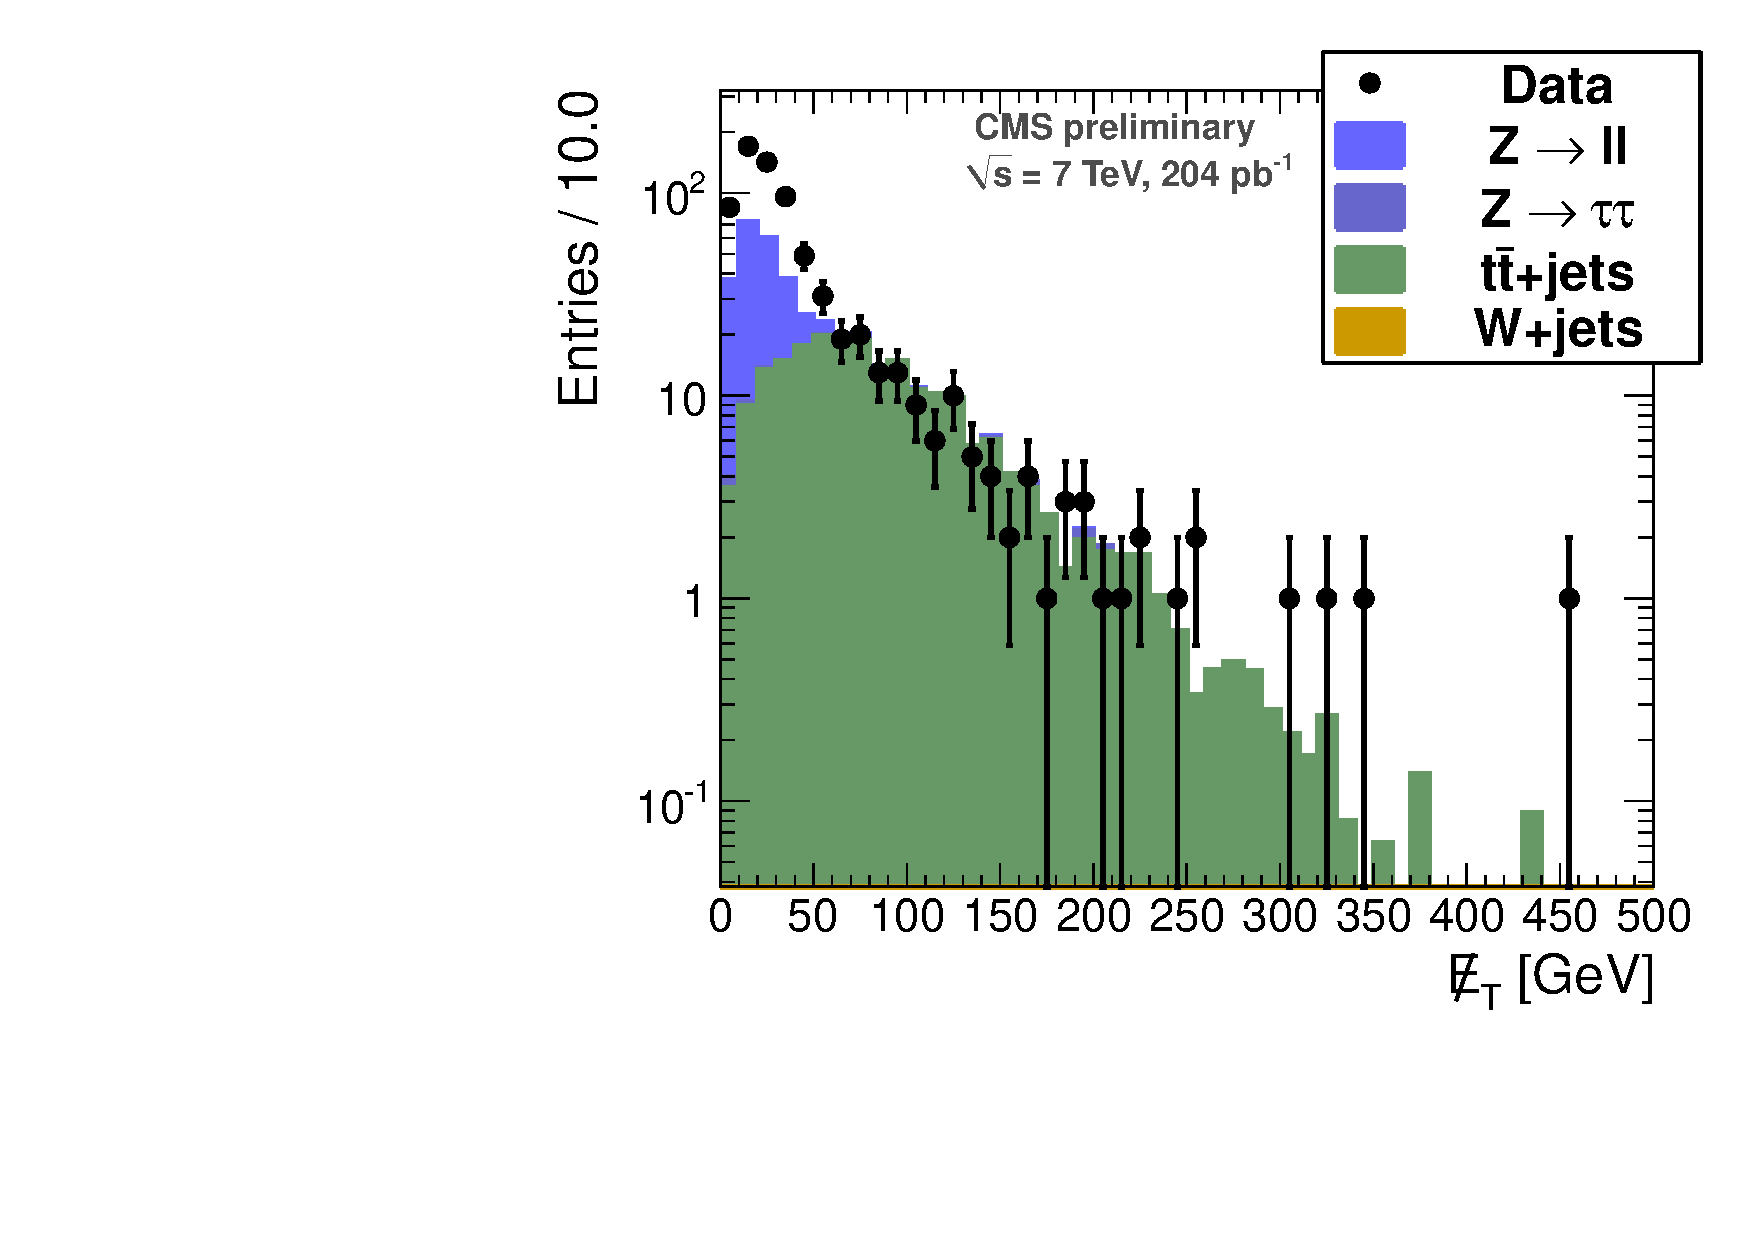
\includegraphics[width=0.79\textwidth]{Summer11_07_MC_pfLeptSusyCuts_Data_MET_HighMET.pdf}}\hfill
  \caption{\MET distribution for all events passing di-lepton selection and satisfy $\HT> 250$~GeV. For the final \MET selection (250)~GeV the selection is dominated by $t\bar{t}$.}
\end{figure}

The \MET distribution after application of the \HT
cut is shown in Fig~\ref{fig:METHighHT} and
the yield split by flavour for a cut at 250~GeV is listed in Tab.~\ref{tab:HighMET}.
It is seen that the yield in data is higher compared 
to simulation for this signal region.

\begin{table}[htb]
\begin{center}
\caption{\label{tab:HighMET}\protect Summary of number of events expected from Monte Carlo simulations in 
the signal region of $H_T> 250$~GeV and $\MET> 250$~GeV. The errors reflect the Monte Carlo (scaled
    to 204~\pbi) statistics only.}
\begin{tabular}{l|ccc|c}
\hline
Process           & $ee$       & $\mu\mu$     & $e\mu$   & total   \\
\hline\hline
$W+\textrm{jets}$ &$0.0 \pm 0.0$&$0.0 \pm 0.0$&$0.0 \pm 0.0$&$0.0 \pm 0.0$\\
$Z\rightarrow ll+\textrm{jets}$&$0.0 \pm 1.97$&$0.0 \pm 1.97$&$0.0 \pm 1.97$&$0.0 \pm 0.27$\\
$Z \rightarrow \tau\tau$&$0.0 \pm 1.0$&$0.0 \pm 1.0$&$0.0 \pm 1.0$&$0.0 \pm 0.27$\\
$t\bar{t}$&$0.4 \pm 0.16$&$1.0 \pm 0.23$&$1.68 \pm 0.28$&$3.08 \pm 0.4$\\
\hline
Total background &$0.4 \pm 2.22$&$1.0 \pm 2.22$&$1.68 \pm 2.23$&$3.08 \pm 0.56$\\
\hline
Data  & 3 & 0 & 3 & 6 \\
\hline\hline
%LM0               &$3.41 \pm 0.17$&$3.91 \pm 0.17$&$4.52 \pm 0.14$&$11.84 \pm 0.42$ \\
%LM1               &$1.64 \pm 0.04$&$2.02 \pm 0.04$&$1.01 \pm 0.03$&$4.64 \pm 0.07$ \\
%\hline
\end{tabular}
\end{center}
\end{table}
